% !TEX program = xelatex
\documentclass{article}
\usepackage{xcolor}
\usepackage{fontspec}
\usepackage{expl3}
\usepackage{xparse}
\usepackage{lmodern}
\usepackage{indentfirst}
\usepackage{censor}
\usepackage{lineno}
\usepackage{titlepic}
\usepackage{blindtext} %This package generates automatic text
\usepackage{epigraph} 
\usepackage{smartdiagram}
\usepackage{float}
\newfontfamily\arial{Arial}

\setmainfont{Latin Modern Roman}

% Fancy chapter styling in an article document
\usepackage{titlesec}
\usepackage{tikz}



% Language setting
% Replace `english' with e.g. `spanish' to change the document language
\usepackage[english]{babel}

% Set page size and margins
% Replace `letterpaper' with `a4paper' for UK/EU standard size
\usepackage[letterpaper,top=2cm,bottom=2cm,left=3cm,right=3cm,marginparwidth=1.75cm]{geometry}

% Useful packages
\usepackage{amsmath}
\usepackage{graphicx}
\usepackage[colorlinks=true]{hyperref}

\graphicspath{ {./assets/} }

% Set TOC depth to include sections and subsections
\setcounter{tocdepth}{2}

\title{Your Deck is Low Skill: \\ A Comprehensive Analysis of Card performance in Clash Royale}
\author{Nathan Yan}
\setlength{\parindent}{20pt}
\begin{document}



\maketitle
\clearpage
\hypersetup{allcolors=black}
\tableofcontents
\hypersetup{allcolors=blue}  % Reset to blue for rest of document
\clearpage

\begin{abstract}
    Clash Royale is a popular mobile strategy game where players build decks of cards to battle against each other in real-time. This report analyzes the performances of both individual cards and overall deck compositions in mid-ladder play using data gathered from Clash Royale's official API. By employing a depth-first search strategy to sample mid-ladder players, this report identifies key cards and strategies that contribute to success in this unique gaming environment. The findings provide insights into effective deck-building strategies and highlight the differences between mid-ladder and top-ladder playstyles.
\end{abstract}

\section{Introduction}
Why do we clash? Simply, we clash to prove our dominance over others. In Clash Royale, players build decks of cards to battle against each other in high-pressure, intense real-time strategy matches. Like Chess, but higher skill and better. Players spend hours meticulously crafting their decks, analyzing card synergies and weaknesses, all in pursuit of sweet victory. But what truly makes a deck powerful? What if there was a more systematic way to evaluate card performance beyond personal preferences? This report aims to uncover the secrets behind card effectiveness in Clash Royale using data-driven analysis. This report focuses not on top ladder, where top decks are well-known\footnote{You can find usage rates and top decks at \href{https://www.deckshop.pro/}{Deck Shop} and many other similiar sites.}, but rather on mid-ladder play, a completely different evironment where players have less optimized decks and where level differences are often pronounced. The best decks at mid-ladder are not the same as those in top-ladder, and this report aims to identify which cards truly shine in this unique context. Many qualitative analyses of mid-ladder decks exist on forums and YouTube, but this report seeks to provide a quantitative perspective on card performance that is able to affirm or refute these claims. The general consensus is that mid-ladder play focuses on simple to play decks that do not require excessive tech, such as precise timings and placements. Additionally, levelling differences also make certain decks more powerful, being able to overpower opponents with sheer stat advantages. For example, while P.E.K.K.A has very few interaction changes when overlevelled, cards like Fireball and Mega Knight gain significant advantages when overlevelled. This report aims to analyze these claims using data gathered from mid-ladder players, providing insights into which cards and strategies are most effective in this environment.

\section{Methodology}

This report was constructed using data entirely gathered using Clash Royale's official API, a robust API that has high rate limits and tons of information on decks and games. While a complete census of top players and their decks is feasible, analyzing mid-ladder play presents unique challenges. Top leaderboards are easily accessible via the API, but mid-ladder data is not as straightforward to obtain. A random sampling approach would be optimal, but the API does not support random sampling of players. Instead, this report employed a DFS (depth-first search) strategy to traverse the player network. Starting from a seed player, the algorithm explored their recent battles, collecting data on their opponents and recursively iterating through the opponents' battles. This method allowed for a large sampling of mid-ladder players, capturing a diverse range of decks and strategies. However, it is not a true random sample, as those with more connections (games played against others) are overrepresented in the sample. I argue that this bias is a non-issue, as this random sampling of \emph{battles} rather than players is more representative of the actual gameplay experience. Players who engage in more battles are more likely to be encountered by others, making their decks and strategies more relevant for analysis. Among the data collected were deck compositions, win rates, game outcomes, and trophies. Evolutions are neglected in this report, as they were rather unwieldy to analyze and some gamemodes do not allow evolutions. 

The Depth First Search began at my personal account at 7,000 trophies, and explored all opponents in recent battles until there were 10,000 unique players sampled. Note that this is \emph{opponents}, and only a few hundred players' battles were sampled. This is a potential limitation that could skew results, but it would only result in an overrepresentation of the type of players that I personally play against, providing a benefit to analysis. The data collection process took approximately 1 hour, with rate limits being the main bottleneck. 10,000 API requests were made, collecting data on 10,000 unique players and their decks. The data was then cleaned and processed using R, with win rates calculated for individual cards and overall deck compositions. However, players with 10,000 trophies are excluded because their trophy count is reset to 10,000 every season, making it a poor indicator of their actual skill. This left me with 7,768 samples.

\section{Results}

\subsection{Sample Analysis}

First, an analysis of the sample as a whole. The trophy distribution of sampled players, as shown in Figure~\ref{fig:trophy_dist} indicates that most players in the sample are clustered around 5,000 to 8,000 trophies, with a tail that extends down to 0 trophies. This suggests that the sample effectively captures mid-ladder players, who typically fall within this trophy range. This distribution also matches the distributions given by official sources, indicating that the sampling method was effective in capturing a representative sample of mid-ladder players. 

\begin{figure}[h]
    \centering
    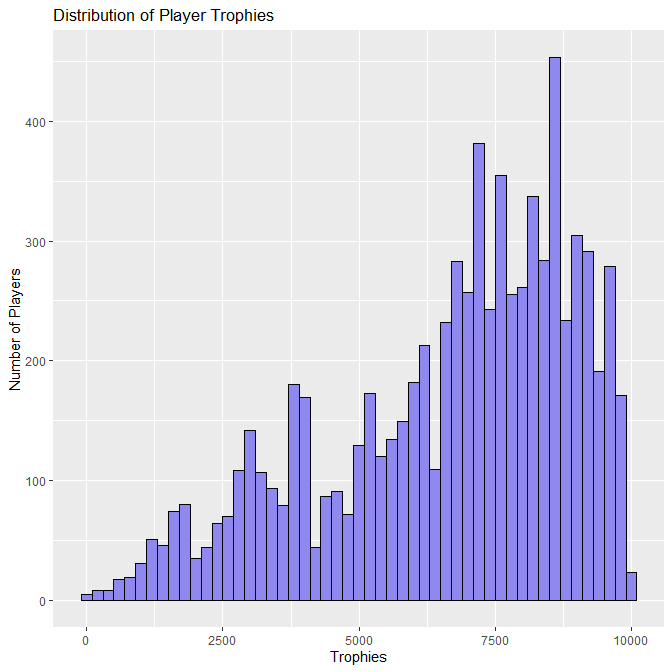
\includegraphics[width=0.7\textwidth]{./assets/trophy_distribution.png}
    \caption{Trophy Distribution of Sampled Players}
    \label{fig:trophy_dist}
\end{figure}

The distribution of win rates across all players is shown in Figure~\ref{fig:winrate_dist}. It appears approximately normal, with a mean win rate of 54\%. A Shapiro-Wilk test, however, indicates that the distribution was not normal and a \hyperref[fig:qq_plot_winrate]{Q-Q plot} displays fat tails, even when only players with over 100 wins are considered. This is slightly higher than the expected 50\% win rate, which could be attributed to the fact that people with very low win rates tend to quit the game, while those with higher win rates continue to play. There is a small bump at around 30\% win rate, which are suspected to be bots. See figure~\ref{fig:winrate_trophy_plot}, which shows a clear bimodal distributions of win rates at low trophies, with win rates converging to around 50\% at higher trophies. The bottom trend line is probably bots, while the top trend line is real players. While efforts can be made to mitigate bot influence, such as filtering out players with low activity, I am too lazy to take these measures. It is important to note that this data also includes low trophy players, which tend to have more extreme win rates. Still, removing players with less than 5000 trophies does not significantly change the distribution. Thus, I saw no need to filter out low trophy players.


\begin{figure}[h]
    \centering
    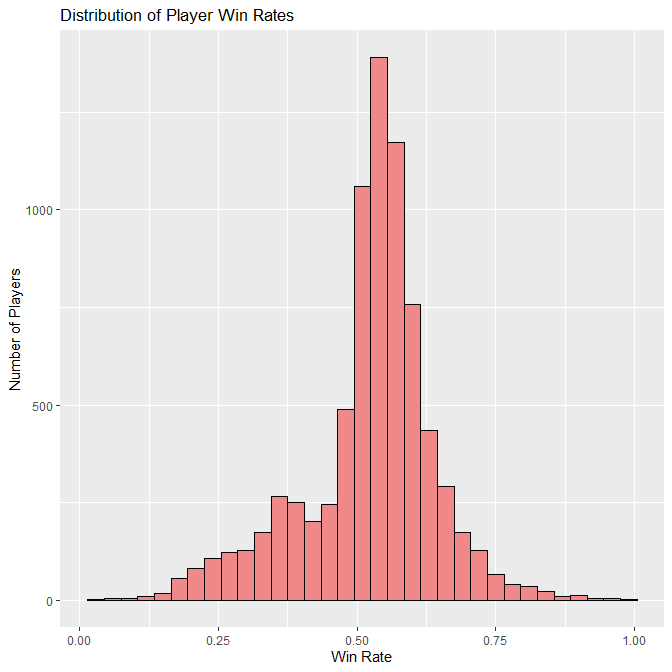
\includegraphics[width=0.7\textwidth]{./assets/winrate_distribution.png}
    \caption{Win Rate Distribution of Sampled Players}
    \label{fig:winrate_dist}
\end{figure}

\begin{figure}[h]
    \centering
    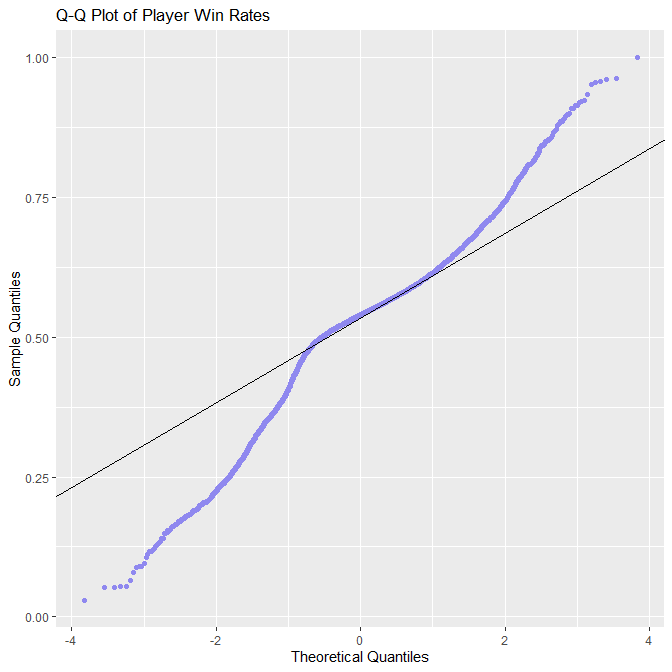
\includegraphics[width=0.7\textwidth]{./assets/qq_plot_winrate.png}
    \caption{Q-Q Plot of Player Win Rates}
    \label{fig:qq_plot_winrate}
\end{figure}

\begin{figure}[h]
    \centering
    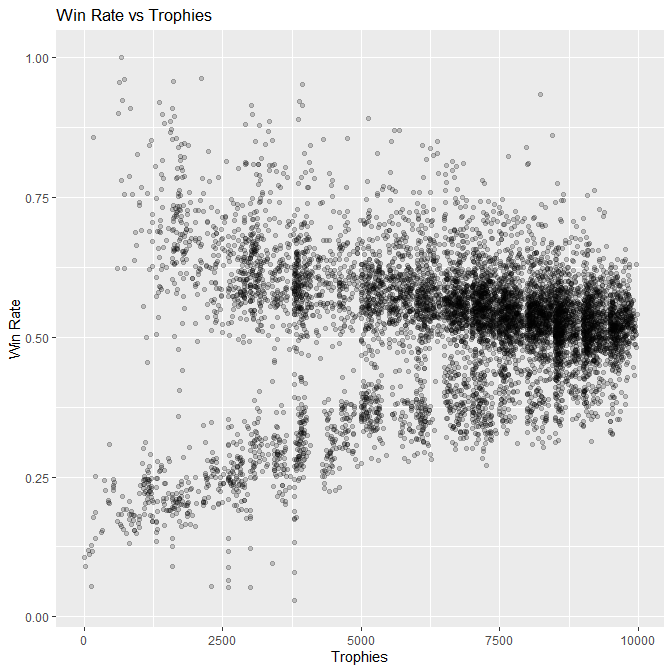
\includegraphics[width=0.7\textwidth]{./assets/winrate_trophy_plot.png}
    \caption{Win Rate vs Trophies of Sampled Players}
    \label{fig:winrate_trophy_plot}
\end{figure}
\clearpage
\subsection{Case Studies}

There are some cards which are notoriously known to be powerful at mid-ladder, such as Mega Knight and Witch. 

\begin{enumerate}
    \item \textbf{Mega Knight} \\
    Mega Knight is definitely the most infamous mid-ladder card, and for good reason. It is a defensive menace, and its splash damage and high health makes it much stronger when overlevelled. Figure~\ref{fig:megaknight_trophy_dist} shows the trophy distributions of players who use Mega Knight versus those who do not. It starts at zero, and as players unlock Mega Knight at around 3,000 trophies, it steadily increases, until it covers about a fourth of all decks in the 6,000 to 10,000 range. This usage is much higher than in top-ladder play, even while Mega Knight is meta. The win rates of Mega Knight users is significantly higher than non-users, with an average win rate of 56.27\% verses the 52.47\% of non-users ($p < 0.01$ using a t-test) in the 6,000-8,000 range. This indicates that often Mega Knight is hard for other mid-ladder players to counter, and that the difference in win rate is not caused by confounding variables such as trophy count. None of this should come as a surprise to any Clash Royale enthusiast.
    \begin{figure}[h]
        \centering
        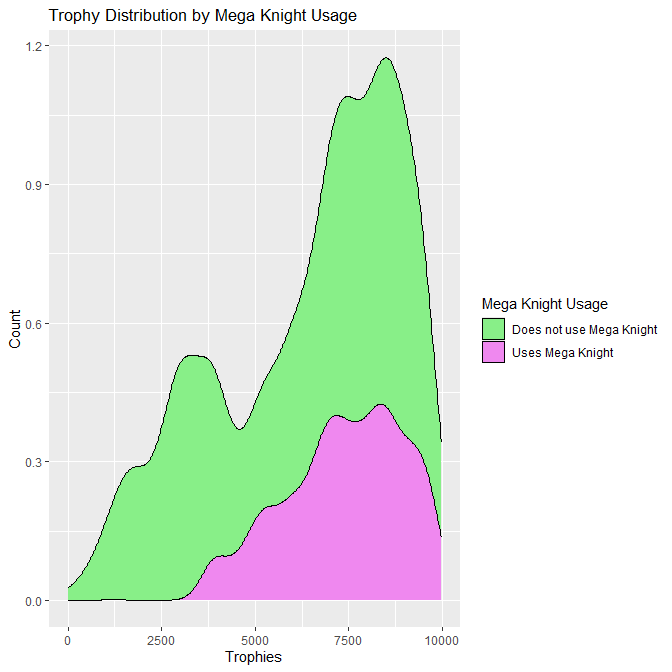
\includegraphics[width=0.7\textwidth]{./assets/megaknight_trophy_distribution.png}
        \caption{Trophy Distribution by Mega Knight Usage}
        \label{fig:megaknight_trophy_dist}
    \end{figure}

    \item \textbf{Giant} \\
    Giant is a bit of an unusual case. Out of all cards, Giant has the lowest overall win rate, sitting at a cool 41\% mean. When you look at the win rates and trophies of Giant users, there is a large clump of them at low trophies with very low win rates, as shown in Figure~\ref{fig:giant_winrate_trophy_plot}. This is probably because bots at low trophies tend to use Giant decks. When low trophy accounts are excluded, Giant users have a mean win rate of 49\%. Still below average, but not as abysmal. 
    \begin{figure}[h]
        \centering
        \includegraphics[width=0.7\textwidth]{./assets/GiantWinRateTrophy.png}
        \caption{Win Rate vs Trophies of Giant Users}
        \label{fig:giant_winrate_trophy_plot}
    \end{figure}
    \item \textbf{Witch} \\
    Witch is the most used card in the sample, standing at a staggering 31.6\% usage rate. This is much higer than top-ladder play, where witch is regarded as a mediocre card. Still, the win rate of Witch users is about average, at 54.7\%. Witch is another splash damage dealer that is difficult for low skill players to counter, especially since overlevelling Witch changes major spell interactions, such as a +2 Witch surviving lightning. Thus, it is no surprise that Witch is so prevalent at mid-ladder play.
\end{enumerate}

\subsection{Regression Analysis}

Next, I performed a regression analysis to identify which cards have the most significant impact on win rates. Each card was given a binary indicator variables representing whether or not it was included in a player's deck. The multiple regression model was then fitted using these indicator variables as predictors and the player's win rate as the response variable. The results of the regression analysis are summarized in Table~\ref{tab:regression_summary}.

\begin{table}[h]
    \centering
    \begin{tabular}{lr}
        \hline
        \textbf{Metric} & \textbf{Value} \\
        \hline
        Multiple R-squared & 0.2024 \\
        Adjusted R-squared & 0.1893 \\
        F-statistic & 15.47 \\
        p-value & $< 2.2 \times 10^{-16}$ \\
        Residual standard error & 0.1071 \\
        Degrees of freedom & 7619 \\
        \hline
    \end{tabular}
    \caption{Summary of Regression Model Statistics}
    \label{tab:regression_summary}
\end{table}

The model achieved a Multiple R-squared of 0.1659 (Adjusted R-squared: 0.1553), indicating that approximately 16.6\% of the variance in win rates can be explained by deck composition alone. The F-statistic of 15.7 with p-value $< 2.2 \times 10^{-16}$ suggests that the overall model is highly significant.

As for dianostic plots (Figure~\ref{fig:regression_diagnostics}), the plots look mostly good, but the distribution in residuals is distinctly fat-tailed. This is a concern, but given the large sample size, the Central Limit Theorem should ensure that the estimates are still valid. THe residuals show no serious outliers, there are no influential points.

\begin{figure}[h]
    \centering
    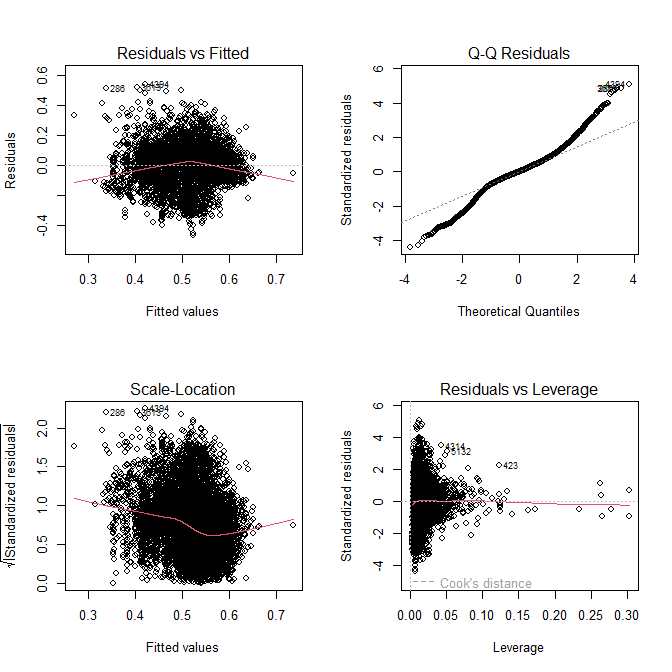
\includegraphics[width=0.9\textwidth]{./assets/regression_diagnostics.png}
    \caption{Diagnostic Plots for Regression Model}
    \label{fig:regression_diagnostics}
\end{figure}

One unusual thing is that most predictors have negative coefficients, and the model is dominated by a few cards with large positive or negative coefficients. These tend to be either win conditions or very rarely used cards. This suggests that higher skill players tend to play more diverse decks that are often off-meta in middle ladder. 

As for the ``best'' deck composition, the model suggests that the optimal deck includes the following:

\begin{itemize}
    \item Barbarian Hut
    \item Hunter
    \item Suspicious Bush
    \item Royal Ghost
    \item Rune Giant
    \item Three Musketeers
    \item Sparky
    \item Golden Knight
\end{itemize}

I did not include evolutions in the model, but since only two cards in this deck have evolutions (Hunter and Royal Ghost), I evolved those. Since there were no interaction terms\footnote{Trying to add them risked overfitting, though there were so many variables that R could not run it anyways.}, this deck's synergy is questionable. After one game, I realized that this deck is actually complete garbage. I elected to switch out Rune Giant for Log just so I dont die immediately to swarms. The deck was slow and expensive, it looks like a beatdown deck but lacks the tank needed to create large pushes, and while it has win conditions in Three Musketeers and Suspicious Bush, they are too slow and easily countered. If allowed to create a deck from the top 20 cards, I was able to create a reasonable hog cycle deck that was able to rack up a few wins.

\section{Conclusion}

While the deck itself was not very useful, the linear model was able to determine the effect of key cards given mid-ladder playstyles. Cards that are easy to use and difficult to counter, such as Mega Knight and Witch, were found to be particularly effective in this environment. The regression analysis provided insights into which cards have the most significant impact on win rates, highlighting the importance of deck composition in mid-ladder play. Overall, this report demonstrates the value of data-driven analysis in understanding card performance in Clash Royale, providing players with valuable insights for deck-building strategies.

\end{document}


